% ============================================================
% 03-proposed-model.tex — V15 Architecture (condensed)
% ============================================================
\section{Proposed Model}
\label{sec:model}

\system{} combines three design principles: centralized coordination, heterogeneous knowledge allocation, and representation-aware evidence routing. A contract-checked supervisor assigns one specialist per query. Depending on the domain, the specialist uses graph traversal for curricula, structured lookup and calculation for fees, or retrieval for narrative policies.

%------------------------------------------------
\subsection{Overall Architecture}
\label{sec:architecture}

Figure~\ref{fig:architecture} illustrates three coordinated tiers: (1)~the Interaction and Centralized Supervisor Tier, (2)~the Domain-Specialized Multi-Agent Core, and (3)~the Heterogeneous Knowledge Storage and Tool Tier.

\begin{figure}[t]
\centering
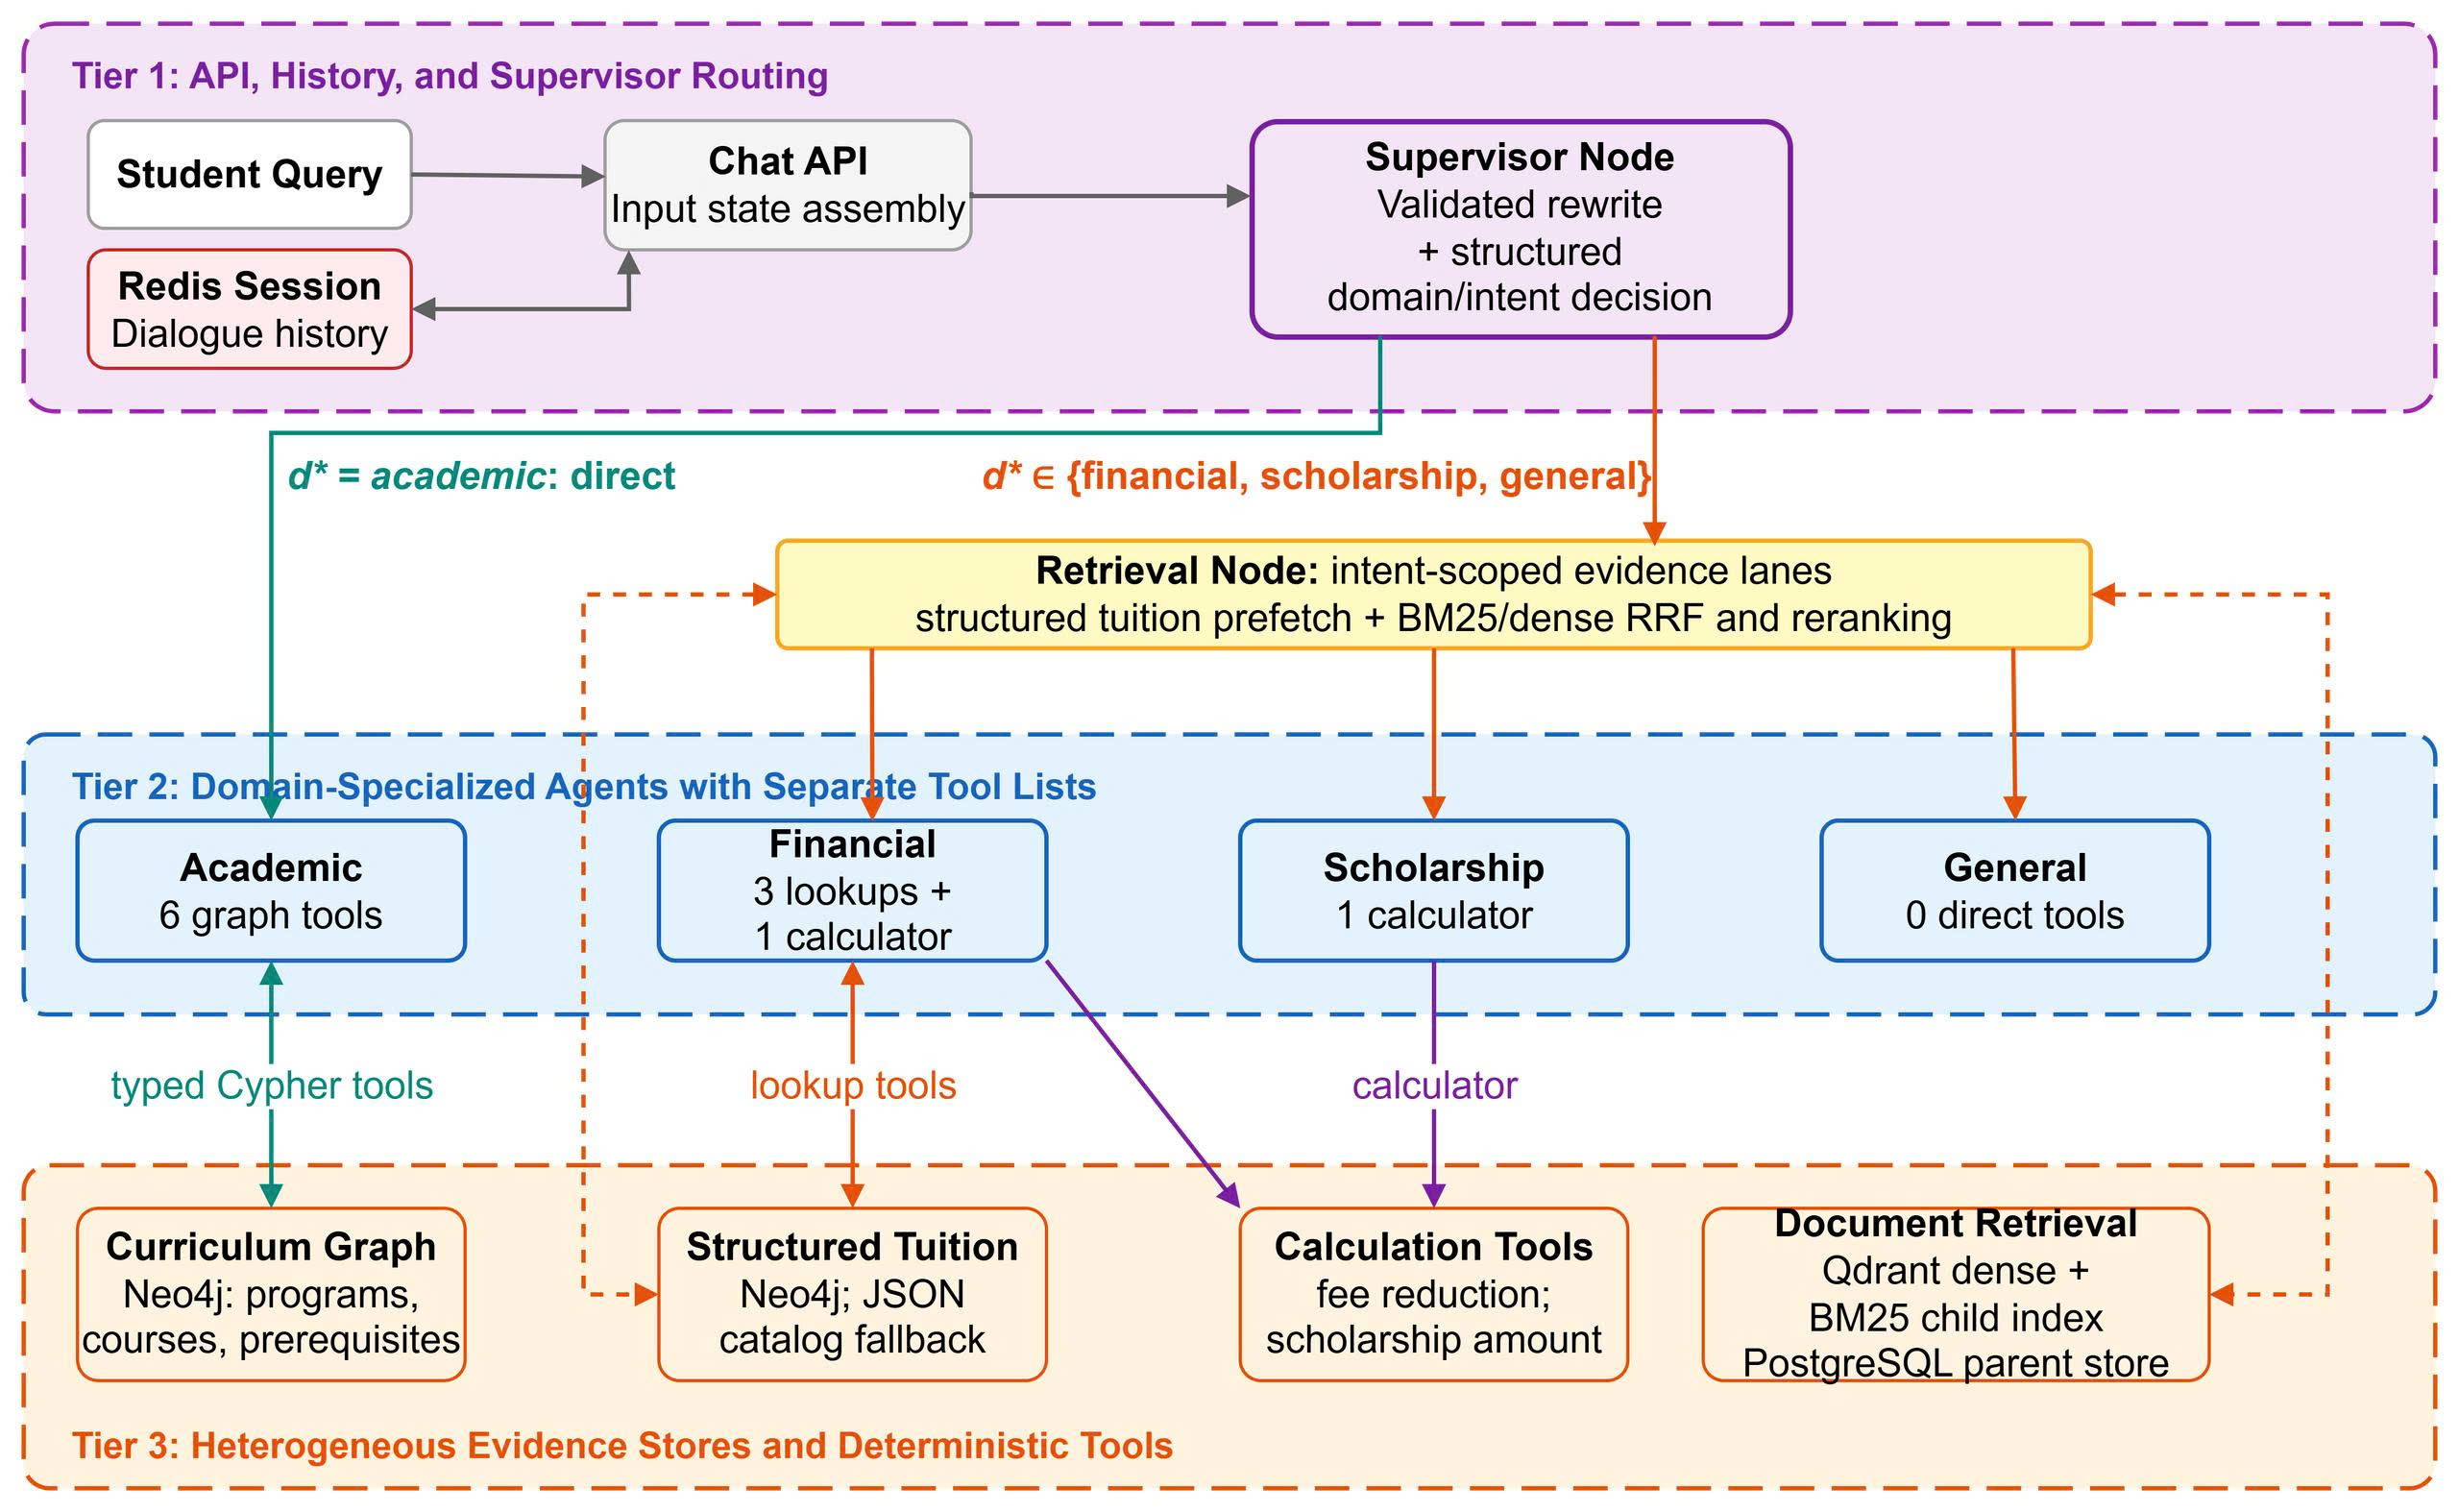
\includegraphics[width=0.88\textwidth]{figures/architecture.jpg}
\Description{Diagram of the three-tier CTU-Chat system architecture. The top tier shows the interaction layer with a centralized supervisor router. The middle tier contains four domain-specialized agents: an academic graph agent connected to Neo4j, a financial agent with deterministic arithmetic tools, a scholarship agent with hybrid retrieval, and a general administrative agent. The bottom tier shows the heterogeneous knowledge storage layer comprising Neo4j graph database, PostgreSQL parent-chunk store, Qdrant vector index, and Redis session history. Solid arrows denote direct tool access and dashed arrows denote retrieval-node evidence acquisition. A contract-repair mechanism validates and may correct the supervisor's routing decision before conditional dispatch.}
\caption{Implemented \system{} architecture. Redis-backed history and validated query rewriting are used in live multi-turn serving; the offline benchmark uses fixed single-turn queries and bypasses these components. The supervisor's structured decision is contract-checked before conditional dispatch. Academic queries enter the graph-enabled agent; other domains pass through intent-scoped retrieval.}
\label{fig:architecture}
\end{figure}

\system{} uses a typed \texttt{AgentState} for rewrites, routes, evidence, and responses. An intent--owner contract checks supervisor output before conditional dispatch: academic queries enter the graph agent; other domains use intent-scoped retrieval. Specialists see only assigned tools and return to \texttt{END} without peer exchanges. The fixed-query benchmark in Section~\ref{sec:exp_setup} bypasses Redis history and query rewriting used in live multi-turn serving.

%------------------------------------------------
\subsection{Neo4j Knowledge Graph and Cypher Tools}
\label{sec:neo4j_graph}

The Neo4j graph is built from 113 curriculum Markdown files representing 111 distinct program codes. The resulting graph stores approximately 7{,}000 nodes across 10 labels: curriculum entities (e.g., \texttt{Program}, \texttt{Course}, \texttt{Block}, \texttt{PLO}, \texttt{PEO}, \texttt{Track}, \texttt{Job}) and tuition entities (\texttt{TuitionFee}, \texttt{TuitionPolicy}, \texttt{ExemptionRate}) connected by over 16{,}000 edges across 13 typed relationships encoding containment, prerequisites, program outcomes, tracks, occupations, tuition, and exemption bases.

The system does not ask the LLM to generate arbitrary Cypher. After the supervisor selects the academic agent, its ReAct policy chooses one of six typed tools and supplies arguments. Each tool normalizes identifiers and calls a fixed, parameterized Cypher query implementing three query classes: \emph{attribute lookup/search} (program codes, names, comparisons), \emph{structural traversal} (prerequisite chains up to ten hops, course intersection, reverse path search), and \emph{structured financial lookup} (tuition, policies, exemption rates). This design binds agent actions to deterministic graph operations, reducing exposure to errors from unconstrained Cypher generation.

%------------------------------------------------
\subsection{Routing and Deterministic Arithmetic}
\label{sec:algorithms}

For a query $q$ and its dialogue predecessor, the supervisor first attempts a validated standalone rewrite, then predicts domain $d_{\mathrm{raw}}$ and intent $\iota_{\mathrm{raw}}$ under a structured schema, falling back to \texttt{general}/\texttt{other} on parsing failure. The ownership contract resolves rule conflicts or incompatible domain--intent pairs. Academic queries proceed directly to the graph agent; other domains build intent-scoped retrieval lanes, with financial queries first attempting Neo4j tuition lookup and then JSON fallback.

\textbf{Deterministic Tuition Arithmetic.}
For fee-reduction requests, the tool \texttt{tinh\_}\allowbreak\texttt{toan\_}\allowbreak\texttt{hoc\_}\allowbreak\texttt{phi} receives three parameters---per-credit tuition $T$, per-credit exemption basis $B$, and exemption percentage $r \in [0, 100]$---and calculates deductible credit amount $D = B \times (r / 100)$ alongside net payable tuition $T_{\mathrm{net}} = \max(0, T - D)$. The tool clamps $T_{\mathrm{net}}$ at zero. The primary contribution is the integration of validated rewriting, constrained routing, and deterministic arithmetic into a unified multi-agent workflow.

%------------------------------------------------
\subsection{Heterogeneous Knowledge Allocation and Hybrid Retrieval}
\label{sec:hybrid_retrieval}

\system{} stores curricula in Neo4j, accesses cohort-specific fees through structured lookup, and retrieves narrative regulations from documents. Financial requests try Neo4j tuition lookup with JSON fallback before the repaired intent selects metadata-filtered retrieval lanes.

For narrative regulations and scholarship criteria, BM25 and Qdrant search 400-character child chunks; parent sections (2,800-char target, 100-char overlap) are loaded from PostgreSQL and fused via RRF: $s_{\mathrm{RRF}}(d)=\sum_{s\in\{\mathrm{bm25},\mathrm{dense}\}}(60+r_s(d))^{-1}$. The full stack pools intent-governed and unfiltered candidates, deduplicates, and reranks with \texttt{bge-reranker-v2-m3}. Scores below 0.20 are removed unless fewer than two candidates remain; graph evidence is added under fixed quotas and up to seven passages are packed for generation.

%------------------------------------------------
\subsection{Cross-Domain Query Handling}
\label{sec:cross_domain}

For cross-domain queries, \system{} uses a single-owner, signal-based evidence-prefetch policy. The supervisor selects an owner by dominant intent; keyword signals add academic-program, academic-regulation, tuition, or scholarship retrieval lanes. The owner uses this evidence without calling another specialist. This bounds execution but may leave a needed tool or source outside the owner's scope. The 20 cross-domain held-out queries test this policy.
